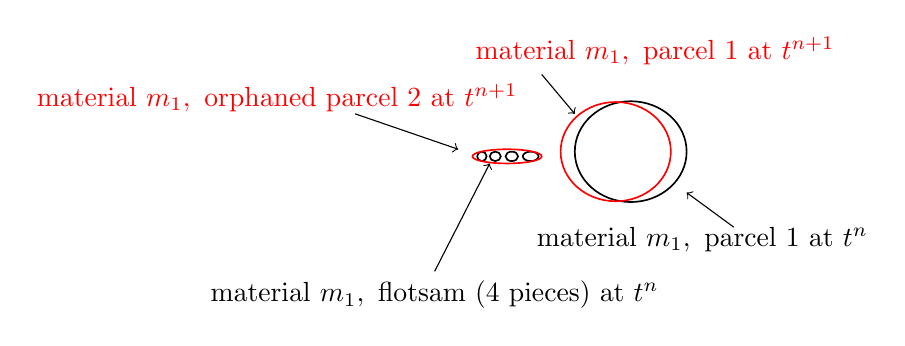
\begin{tikzpicture}
  \draw[semithick] (0.47,1.46) ellipse [x radius=0.07cm, y radius=0.06cm];
  \draw[semithick] (0.68,1.46) ellipse [x radius=0.08cm, y radius=0.06cm];
  \draw[semithick] (0.3,1.46) circle (0.06cm);
  \draw[semithick] (0.92,1.46) ellipse [x radius=0.1cm, y radius=0.06cm];
  \draw[semithick] (2.19,1.52) ellipse [x radius=0.71cm, y radius=0.64cm];


\node at (3.1,0.4){$\textcolor{black}{ \mbox{material } m_{1},\mbox{ parcel } 1 \mbox{ at } t^{n}}$};




\node at (2.5,2.8){$\textcolor{red}{ \mbox{material } m_{1},\mbox{ parcel } 1 \mbox{ at } t^{n+1}}$};



\node (node1) at (-0.3,-0.3){$\textcolor{black}{ \mbox{material } m_{1},\mbox{ flotsam (4 pieces)} \mbox{ at } t^{n}}$};


\node at (-2.3,2.2){$\textcolor{red}{ \mbox{material } m_{1},\mbox{ orphaned parcel } 2 \mbox{ at } t^{n+1}}$};



  \draw[semithick, red] (2,1.52) ellipse [x radius=0.7cm, y radius=0.63cm];
  \draw[red, semithick] (0.62,1.46) ellipse [x radius=0.44cm, y radius=0.09cm];
  \draw[->] (3.5,0.56) -- (2.9,1);
  \draw[->] (1.06,2.5) -- (1.48,2);
  \draw[->] (node1.north) -- (0.4,1.37);
  \draw[->] (-1.31,2) -- (0,1.55);
\end{tikzpicture}